\documentclass{beamer}
\usetheme{Dresden}
\usecolortheme{whale}
\usepackage[utf8]{inputenc}
\usepackage[T1]{fontenc}
\usepackage{ragged2e}
\usepackage{amssymb}
\usepackage{booktabs}
\usepackage{graphicx}
\usepackage{mathtools}
\usepackage{amsmath}
\usepackage{multicol}
\usepackage{listings}
\usepackage{tikz}
\usetikzlibrary{arrows.meta, positioning, shapes.geometric, fit, backgrounds,
                calc, decorations.pathreplacing}

\newcommand{\nt}{$\underline{\text{Note}}:$ }
\newcommand{\nll}{\\\vspace{2ex}}

\graphicspath{ {images/} }

\lstset{
    basicstyle=\ttfamily\scriptsize,
    keywordstyle=\color{blue!70!black},
    commentstyle=\color{gray},
    breaklines=true,
    frame=single,
    backgroundcolor=\color{gray!5},
}

\title[Voice Scribe v4]{Voice Scribe v4\\Real-Time Streaming Ingestion}
\author[J. Yanez]{Johnraymond Yanez}
\institute[Voice Scribe]{Voice Scribe}
\date{Planning: July 2026 --- protocol locked at design review (\texttt{docs/v4/protocol.md})}

\begin{document}


% -- Title -----------------------------------------------------------------
\begin{frame}
\small{\titlepage}
\end{frame}


% -- Overview --------------------------------------------------------------
\begin{frame}{Overview}
    \begin{itemize}
        \item \textbf{The Latency Problem} --- where the 1.2--1.5\,s actually goes
        \item \textbf{Streaming Serving} --- overlap inference with speech
        \item \textbf{Why Whisper Cannot Stream} --- and the policy layer that fakes it
        \item \textbf{LocalAgreement} --- the serving loop, instance to instance
        \item \textbf{Session Architecture} --- protocol, ring buffer, decode ticks
        \item \textbf{Tunables \& Targets} --- five knobs, four measured numbers
        \item \textbf{Hardware Cost} --- v3 vs.\ v4, the compute premium justified
        \item \textbf{Serving Vocabulary} --- what this milestone teaches
        \item \textbf{Plan} --- v4.0--v4.2, testing, gate
    \end{itemize}
\end{frame}


% =========================================================================
\section{The Problem}
% =========================================================================

\begin{frame}{v2.1 ``Streaming'' Is Output-Only}
    \small
    The existing WebSocket path streams \emph{results out}, never \emph{audio in}:

    \vspace{0.4em}
    \begin{enumerate}\setlength{\itemsep}{2pt}
        \item Client VAD waits for a \textbf{complete utterance} (\texttt{onSpeechEnd})
        \item WAV encode $\rightarrow$ \textbf{new WebSocket per utterance} $\rightarrow$
              whole blob in one message
        \item Server writes a temp file $\rightarrow$ ffmpeg transcode $\rightarrow$
              \textbf{full-clip inference}
        \item Only the \emph{segments} stream back incrementally
    \end{enumerate}

    \vspace{0.5em}
    \begin{block}{The observation}
        Every stage begins \emph{after} the user stops speaking. The GPU is idle for
        the entire duration of speech --- the one window in which inference could
        have been free.
    \end{block}
\end{frame}


\begin{frame}{Current Serving Timeline}
    \begin{center}
    \resizebox{\textwidth}{!}{%
    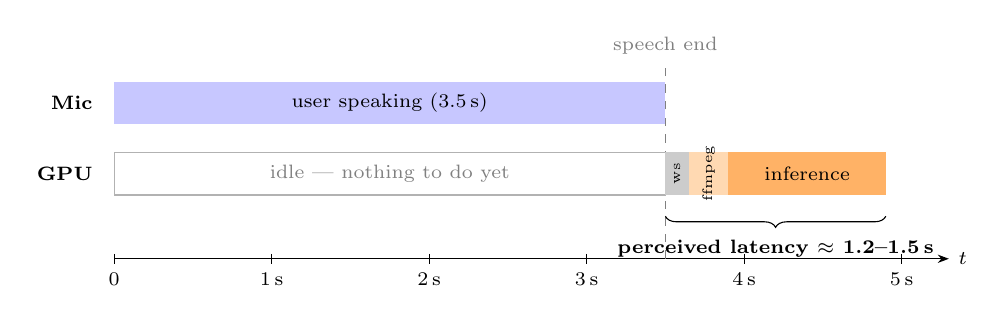
\begin{tikzpicture}[xscale=1.0, yscale=0.9, every node/.style={font=\scriptsize}]
        % time axis (1 unit = 0.5 s)
        \draw[-{Stealth[length=4pt]}] (0,-0.15) -- (10.6,-0.15) node[right]{$t$};
        \foreach \x/\l in {0/0, 2/1\,s, 4/2\,s, 6/3\,s, 8/4\,s, 10/5\,s}
            \draw (\x,-0.08) -- (\x,-0.22) node[below]{\l};

        % row labels
        \node[anchor=east] at (-0.15, 2.05) {\textbf{Mic}};
        \node[anchor=east] at (-0.15, 1.05) {\textbf{GPU}};

        % speech bar: 0 - 3.5 s  -> 0 - 7 units
        \fill[blue!22] (0,1.75) rectangle (7,2.35);
        \node at (3.5,2.05) {user speaking (3.5\,s)};
        \draw[dashed, gray] (7,-0.15) -- (7,2.6);
        \node[gray, anchor=south] at (7,2.6) {speech end};

        % GPU idle: 0 - 3.5 s
        \draw[gray!60] (0,0.75) rectangle (7,1.35);
        \node[gray] at (3.5,1.05) {idle --- nothing to do yet};

        % pipeline after stop: connect/encode 0.15s, transcode 0.25s, inference 1.0s
        \fill[gray!40]   (7.0,0.75) rectangle (7.3,1.35);
        \fill[orange!30] (7.3,0.75) rectangle (7.8,1.35);
        \fill[orange!60] (7.8,0.75) rectangle (9.8,1.35);
        \node at (8.8,1.05) {inference};
        \node[rotate=90, font=\tiny] at (7.15,1.05) {ws};
        \node[rotate=90, font=\tiny] at (7.55,1.05) {ffmpeg};

        % perceived latency brace
        \draw[decorate, decoration={brace, mirror, amplitude=4pt}]
            (7,0.45) -- (9.8,0.45)
            node[midway, below=5pt]{\textbf{perceived latency $\approx$ 1.2--1.5\,s}};
    \end{tikzpicture}%
    }
    \end{center}

    \vspace{0.2em}
    \footnotesize
    All useful work is serialized \emph{after} speech end. Inference time scales with
    utterance length, so longer utterances feel \emph{worse}, not better.
\end{frame}


\begin{frame}{Streaming Serving Timeline}
    \begin{center}
    \resizebox{\textwidth}{!}{%
    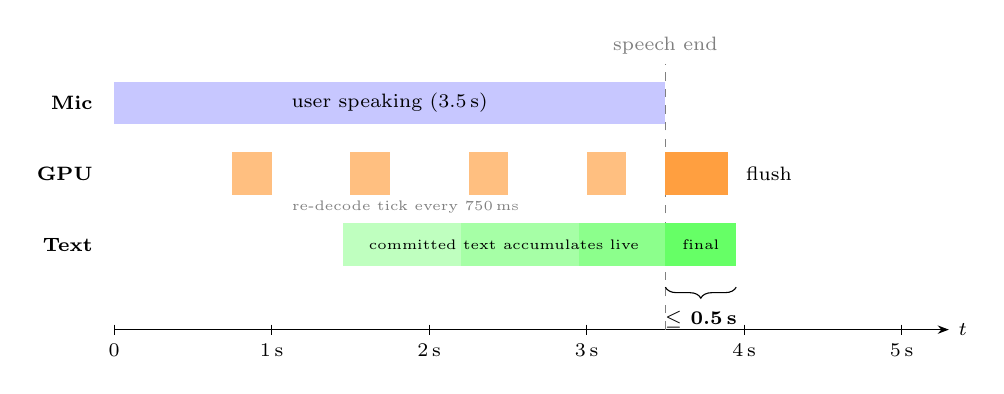
\begin{tikzpicture}[xscale=1.0, yscale=0.9, every node/.style={font=\scriptsize}]
        % time axis
        \draw[-{Stealth[length=4pt]}] (0,-0.15) -- (10.6,-0.15) node[right]{$t$};
        \foreach \x/\l in {0/0, 2/1\,s, 4/2\,s, 6/3\,s, 8/4\,s, 10/5\,s}
            \draw (\x,-0.08) -- (\x,-0.22) node[below]{\l};

        % row labels
        \node[anchor=east] at (-0.15, 3.05) {\textbf{Mic}};
        \node[anchor=east] at (-0.15, 2.05) {\textbf{GPU}};
        \node[anchor=east] at (-0.15, 1.05) {\textbf{Text}};

        % speech bar: 0 - 3.5 s
        \fill[blue!22] (0,2.75) rectangle (7,3.35);
        \node at (3.5,3.05) {user speaking (3.5\,s)};
        \draw[dashed, gray] (7,-0.15) -- (7,3.6);
        \node[gray, anchor=south] at (7,3.6) {speech end};

        % decode ticks every 750 ms -> every 1.5 units, width ~0.5
        \foreach \x in {1.5, 3.0, 4.5, 6.0}
            \fill[orange!50] (\x,1.75) rectangle (\x+0.5,2.35);
        \node at (4.2,2.55) {};
        % flush decode after stop
        \fill[orange!75] (7.0,1.75) rectangle (7.8,2.35);
        \node[anchor=west] at (7.9,2.05) {flush};
        \node[font=\tiny, gray] at (3.7,1.58) {re-decode tick every 750\,ms};

        % committed text growing
        \fill[green!25] (2.9,0.75) rectangle (4.4,1.35);
        \fill[green!35] (4.4,0.75) rectangle (5.9,1.35);
        \fill[green!45] (5.9,0.75) rectangle (7.0,1.35);
        \fill[green!60] (7.0,0.75) rectangle (7.9,1.35);
        \node[font=\tiny] at (4.95,1.05) {committed text accumulates live};
        \node[font=\tiny] at (7.45,1.05) {final};

        % latency brace
        \draw[decorate, decoration={brace, mirror, amplitude=4pt}]
            (7,0.45) -- (7.9,0.45)
            node[midway, below=5pt]{\textbf{$\leq$ 0.5\,s}};
    \end{tikzpicture}%
    }
    \end{center}

    \vspace{0.2em}
    \footnotesize
    Inference overlaps speech. By speech end, most of the transcript is already
    committed; the flush decodes only the short uncommitted tail. Perceived latency
    is now \emph{independent of utterance length}.
\end{frame}


% =========================================================================
\section{The Policy Layer}
% =========================================================================

\begin{frame}{Why Whisper Cannot Stream Natively}
    \footnotesize
    \textbf{Whisper is an offline model.} Encoder--decoder over a 30\,s window;
    you cannot feed it one frame and get one token. Feeding it a growing buffer
    na\"ively gives a \emph{different} hypothesis every pass --- text that rewrites
    itself is unusable for dictation.

    \vspace{0.3em}
    \textbf{Two ways out:}
    \begin{enumerate}\setlength{\itemsep}{2pt}
        \item Switch to a natively-streaming architecture (transducer / RNN-T,
              Kyutai STT) --- \emph{rejected}: abandons the proven
              \texttt{large-v3} accuracy stack
        \item Keep the model, add a \textbf{serving policy layer}: paced re-decode
              of a rolling buffer + a rule for which prefix is stable enough to
              commit --- \emph{chosen}
    \end{enumerate}

    \vspace{0.3em}
    \begin{block}{\footnotesize The key asymmetry}
        \footnotesize
        In a \emph{batch} pipeline, overlapping windows are equally informed ---
        you stitch or blend them. In a \emph{streaming} pipeline every new decode
        sees strictly more context: the newest hypothesis \textbf{supersedes} the
        old one. The only question: \emph{which prefix is stable enough to commit?}
    \end{block}
\end{frame}


\begin{frame}{LocalAgreement --- Instance to Instance}
    \begin{center}
    \resizebox{\textwidth}{!}{%
    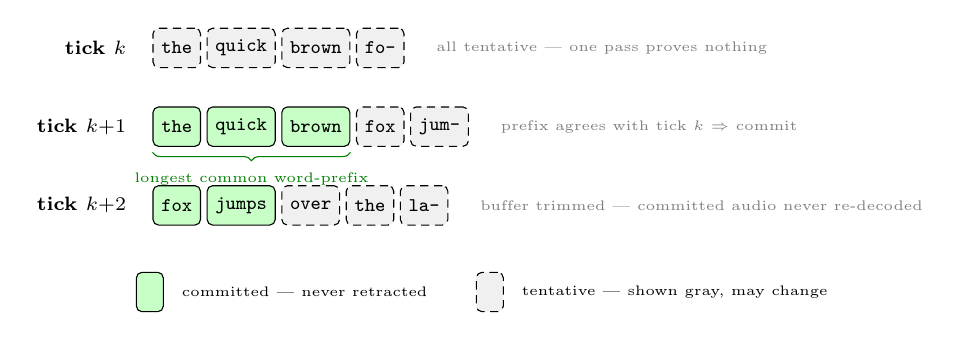
\begin{tikzpicture}[
        node distance=2pt,
        word/.style={draw, rounded corners=2pt, font=\scriptsize\ttfamily,
                     minimum height=0.5cm, inner sep=3pt},
        cmt/.style={word, fill=green!22},
        tn/.style={word, fill=gray!12, densely dashed},
        rowlbl/.style={font=\scriptsize\bfseries, anchor=east},
        ann/.style={font=\tiny, gray},
    ]
        % --- tick k ---
        \node[rowlbl] (r1) at (0,0) {tick $k$};
        \node[tn, right=6pt of r1] (a1) {the};
        \node[tn, right=of a1] (a2) {quick};
        \node[tn, right=of a2] (a3) {brown};
        \node[tn, right=of a3] (a4) {fo-};
        \node[ann, right=8pt of a4] {all tentative --- one pass proves nothing};

        % --- tick k+1 ---
        \node[rowlbl] (r2) at (0,-1.0) {tick $k{+}1$};
        \node[cmt, right=6pt of r2] (b1) {the};
        \node[cmt, right=of b1] (b2) {quick};
        \node[cmt, right=of b2] (b3) {brown};
        \node[tn, right=of b3] (b4) {fox};
        \node[tn, right=of b4] (b5) {jum-};
        \node[ann, right=8pt of b5] {prefix agrees with tick $k$ $\Rightarrow$ commit};

        % --- tick k+2 ---
        \node[rowlbl] (r3) at (0,-2.0) {tick $k{+}2$};
        \node[cmt, right=6pt of r3] (c1) {fox};
        \node[cmt, right=of c1] (c2) {jumps};
        \node[tn, right=of c2] (c3) {over};
        \node[tn, right=of c3] (c4) {the};
        \node[tn, right=of c4] (c5) {la-};
        \node[ann, right=8pt of c5] {buffer trimmed --- committed audio never re-decoded};

        % brace under committed region of row 2
        \draw[decorate, decoration={brace, mirror, amplitude=3pt}, green!50!black]
            ($(b1.south west)+(0,-2pt)$) -- ($(b3.south east)+(0,-2pt)$)
            node[midway, below=4pt, font=\tiny, green!50!black]
            {longest common word-prefix};

        % legend
        \node[cmt, anchor=west] (lg1) at (0,-3.1) {\phantom{x}};
        \node[font=\tiny, right=3pt of lg1] (lgt1) {committed --- never retracted};
        \node[tn, right=14pt of lgt1] (lg2) {\phantom{x}};
        \node[font=\tiny, right=3pt of lg2] {tentative --- shown gray, may change};
    \end{tikzpicture}%
    }
    \end{center}

    \vspace{0.15em}
    \footnotesize
    Agreement-across-time replaces confidence stitching. Every policy element either
    \textbf{commits or withholds --- none revises}: the word-probability floor and the
    buffer-edge guard only withhold; agreement and holdback force-commit only commit.
    Force-commit (after \texttt{MAX\_HOLDBACK\_TICKS}) bounds latency at a stated cost:
    it converts a visible flicker into a possible \emph{invisible permanent error} ---
    hence the gate also measures force-commit rate and WER, not just retractions.
\end{frame}


\begin{frame}{Session Architecture}
    \begin{center}
    \resizebox{!}{0.74\textheight}{%
    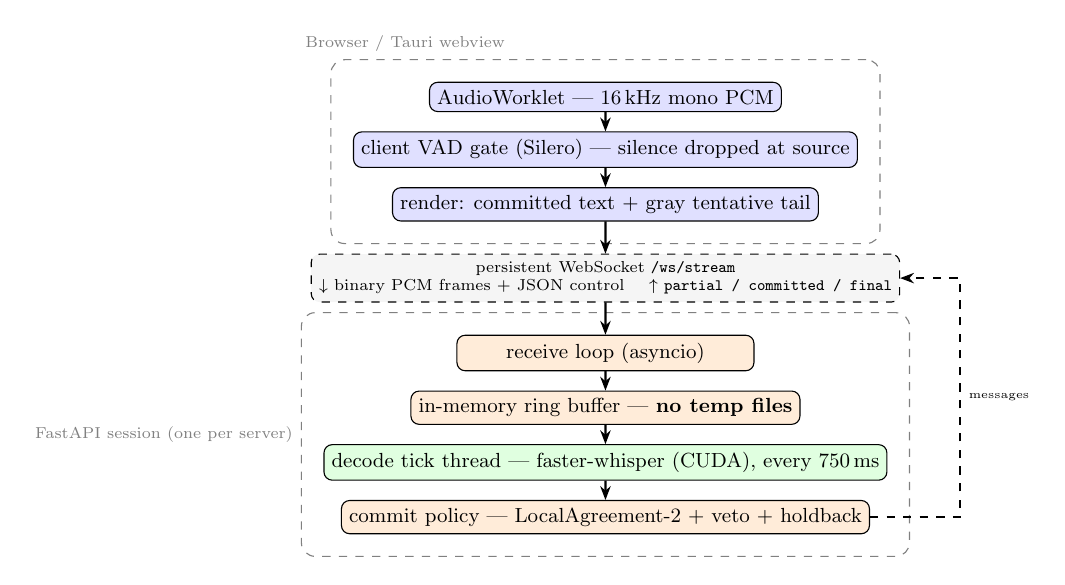
\begin{tikzpicture}[scale=0.82, every node/.style={transform shape},
        node distance=0.3cm,
        box/.style={draw, rounded corners=3pt, minimum width=4.6cm,
                    minimum height=0.45cm, font=\small, align=center},
        client/.style={box, fill=blue!12},
        server/.style={box, fill=orange!15},
        gpu/.style={box, fill=green!12},
        wire/.style={draw, rounded corners=3pt, minimum width=3.8cm,
                    minimum height=0.45cm, font=\scriptsize, align=center,
                    fill=gray!8, dashed},
        arr/.style={-{Stealth[length=5pt]}, thick},
        boundary/.style={draw, dashed, rounded corners=5pt, gray, inner sep=8pt},
    ]
        % client side
        \node[client] (worklet) {AudioWorklet --- 16\,kHz mono PCM};
        \node[client, below=0.3cm of worklet] (vad) {client VAD gate (Silero) --- silence dropped at source};
        \node[client, below=0.3cm of vad] (render) {render: committed text + gray tentative tail};

        \begin{scope}[on background layer]
            \node[boundary, fit=(worklet)(vad)(render),
                  label={[font=\scriptsize, text=gray]above left:Browser / Tauri webview}] {};
        \end{scope}

        % wire
        \node[wire, below=0.5cm of render] (ws)
              {persistent WebSocket \texttt{/ws/stream}\\
               $\downarrow$ binary PCM frames + JSON control
               \quad $\uparrow$ \texttt{partial / committed / final}};

        % server side
        \node[server, below=0.5cm of ws] (recv) {receive loop (asyncio)};
        \node[server, below=0.3cm of recv] (ring) {in-memory ring buffer --- \textbf{no temp files}};
        \node[gpu, below=0.3cm of ring] (decode) {decode tick thread --- faster-whisper (CUDA), every 750\,ms};
        \node[server, below=0.3cm of decode] (policy) {commit policy --- LocalAgreement-2 + veto + holdback};

        \begin{scope}[on background layer]
            \node[boundary, fit=(recv)(ring)(decode)(policy),
                  label={[font=\scriptsize, text=gray]left:FastAPI session (one per server)}] {};
        \end{scope}

        \draw[arr] (worklet) -- (vad);
        \draw[arr] (vad) -- (render);
        \draw[arr] (render) -- (ws);
        \draw[arr] (ws) -- (recv);
        \draw[arr] (recv) -- (ring);
        \draw[arr] (ring) -- (decode);
        \draw[arr] (decode) -- (policy);
        \draw[arr, dashed] (policy.east) -- ++(1.4,0) |-
              node[near start, right, font=\tiny]{messages} (ws.east);
    \end{tikzpicture}%
    }
    \end{center}
\end{frame}


% =========================================================================
\section{Tunables \& Targets}
% =========================================================================

\begin{frame}{The Five Tunables}
    \begin{table}
    \centering\scriptsize
    \begin{tabular}{@{} l p{5.4cm} l @{}}
        \toprule
        \textbf{Parameter} & \textbf{Meaning} & \textbf{Initial} \\
        \midrule
        \texttt{DECODE\_TICK\_MS} & Re-decode pacing; main latency/compute dial.
            Commit lag $\approx$ 2 ticks. & 750\,ms \\
        \texttt{WORD\_PROB\_FLOOR} & Veto (withhold-only): word below this
            \texttt{word.probability} never commits. & 0.5 \\
        \texttt{EDGE\_GUARD\_S} & Veto: never commit a word ending within this
            distance of the buffer end (edge hallucinations agree across
            ticks). & 0.6\,s \\
        \texttt{MAX\_HOLDBACK\_TICKS} & Force-commit ceiling, frontier-anchored;
            bounds worst-case latency. & 6 \\
        \texttt{MAX\_UNCOMMITTED\_S} & Uncommitted cap; window invariant
            $3 + 24 + 3 \leq 30$\,s (left context + uncommitted + safety). & 24\,s \\
        \bottomrule
    \end{tabular}
    \end{table}

    \vspace{-0.2em}
    \scriptsize
    Plus one non-tunable rule: \textbf{VAD flush} --- speech end is ground truth.
    Decode the remaining buffer once, finalize everything. This bounds
    finalization latency in practice.

    \begin{block}{\footnotesize The trade, stated honestly}
        \footnotesize
        Each second of audio is decoded 3--5$\times$: compute is spent to buy
        latency. Right trade on a dedicated local GPU --- but
        \emph{measured and reported}, not assumed.
    \end{block}
\end{frame}


\begin{frame}{Latency Targets --- the Gate Is a Measurement}
    \begin{table}
    \centering\footnotesize
    \begin{tabular}{@{} l l l @{}}
        \toprule
        \textbf{Metric} & \textbf{Today} & \textbf{v4 target} \\
        \midrule
        First partial visible (from speech onset) & n/a & $\leq$ 1.5\,s \\
        Final transcript (from \texttt{flush} receipt)\textsuperscript{*} & $\sim$1.2--1.5\,s & $\leq$ 0.5\,s \\
        Committed-text retractions & n/a & 0 (by construction) \\
        Force-commit rate / committed WER & n/a & $<$5\,\% / $<$3\,\% \\
        Tick occupancy (decode\,/\,tick budget) & n/a & p95 $\leq$ 0.7 \\
        GPU re-decode overhead & 1$\times$ & measured, reported \\
        \bottomrule
    \end{tabular}
    \end{table}

    \vspace{0.5em}
    \footnotesize
    \textbf{Measurement harness ships with the endpoint:}\\
    \texttt{ops/scripts/stream\_bench.py} replays a WAV over \texttt{/ws/stream}
    at real-time pace; reports first-partial latency, finalization latency,
    commit-lag distribution, retraction count.

    \vspace{0.3em}
    \scriptsize
    \textsuperscript{*}\,Client VAD detection lag (\texttt{redemptionMs}) is a separate,
    additive v4.1 number --- bench and live measure different anchors by design.
    \nt tuning without instrumentation is guessing. The harness is v4.0 scope,
    not an afterthought --- same discipline as v1's smoke-test latency record.
\end{frame}


\begin{frame}{Hardware Cost Justification --- v3 vs.\ v4}
    \small
    Streaming spends compute to buy latency. The premium is \emph{quantified},
    not asserted: \texttt{stream\_bench} runs the \textbf{same audio} through
    both paths and publishes the comparison.

    \vspace{0.3em}
    \begin{table}
    \centering\scriptsize
    \resizebox{\textwidth}{!}{%
    \begin{tabular}{@{} l l l @{}}
        \toprule
        \textbf{Measured per run} & \textbf{v3 one-shot (baseline)} & \textbf{v4 streaming} \\
        \midrule
        Decode-seconds per audio-second & $\sim$1$\times$ & expected 3--5$\times$ \\
        GPU duty cycle (\texttt{nvidia-smi}) & idle until speech end & sustained during speech \\
        Peak VRAM & measured & measured \\
        Per-tick decode time (RTF) & n/a & must stay $<1$ \\
        Finalization latency & $\sim$1.2--1.5\,s & $\leq$ 0.5\,s \\
        \bottomrule
    \end{tabular}%
    }
    \end{table}

    \vspace{0.3em}
    \begin{block}{\footnotesize The justification, stated as a sentence}
        \footnotesize
        ``An $X\times$ compute premium bought $Y$\,ms of perceived latency.''
        $X$ outside the 3--5$\times$ envelope is a tuning finding (tick too
        fast, buffer trim broken) --- not a number to quietly accept. Per-tick
        RTF $\geq 1$ means the buffer grows without bound: a correctness
        failure, not a performance quirk.
    \end{block}
\end{frame}


% =========================================================================
\section{Serving Vocabulary}
% =========================================================================

\begin{frame}{What This Milestone Teaches (Field Vocabulary)}
    \vspace{-0.3em}
    \begin{table}
    \centering\scriptsize
    \begin{tabular}{@{} l p{6.2cm} @{}}
        \toprule
        \textbf{Term} & \textbf{Where it appears in v4} \\
        \midrule
        Session & One connection = one stateful stream with its own buffer
                  and decode loop \\
        First-token latency & First-partial latency --- the streaming world's
                  headline metric \\
        Finalization latency & Speech end $\rightarrow$ final text; what the
                  user actually feels \\
        RTF (real-time factor) & Decode time $\div$ audio duration; must stay
                  $<1$ per tick or the buffer grows unboundedly \\
        Commit / stability policy & LocalAgreement + veto + holdback --- the
                  quality/latency contract \\
        Backpressure & What happens when decode ticks fall behind frame
                  arrival (skip ticks, never queue unboundedly) \\
        Graceful degradation & Stream fails $\rightarrow$ one-shot WS
                  $\rightarrow$ HTTP POST; three-deep fallback chain \\
        \bottomrule
    \end{tabular}
    \end{table}

    \scriptsize
    Contrast worth knowing: LLM serving batches \emph{across users} (continuous
    batching); a local voice tool batches \emph{across time} for one user. Same
    discipline --- schedulers, budgets, SLOs --- different axis. Streaming ASR
    policy layers, session management, and latency instrumentation are exactly
    the skills the voice-systems field hires for.
\end{frame}


% =========================================================================
\section{Plan}
% =========================================================================

\begin{frame}{Sub-Milestones}
    \footnotesize
    \begin{table}
    \centering\scriptsize
    \begin{tabular}{@{} l p{7.2cm} @{}}
        \toprule
        \textbf{Milestone} & \textbf{Deliverable} \\
        \midrule
        v4.0 & Backend session loop per \texttt{docs/v4/protocol.md}:
               \texttt{/ws/stream}, decode ticks, LocalAgreement pure core,
               VAD flush. Contract + privacy diagram updated. Driven by
               \texttt{stream\_bench}; no frontend changes \\
        v4.1 & Frontend: persistent session, \texttt{onFrameProcessed} tap +
               pre-roll replay, partial-vs-committed rendering, degrade
               ladder. \texttt{state-machine.mmd} \emph{before} code \\
        v4.2 & Fast path on committed text --- \textbf{copy only}
               (review-locked) + tuning against \texttt{stream\_bench} \\
        \bottomrule
    \end{tabular}
    \end{table}

    \vspace{0.1em}
    \textbf{Testing folded into each sub-milestone:}
    \begin{itemize}\setlength{\itemsep}{0pt}
        \item Commit policy as \textbf{pure functions} --- synthetic hypothesis
              sequences, no GPU, no WebSocket
        \item Session tests: model-mocking pattern, each names its clause
        \item vitest: partial rendering, retraction, fallback, teardown
    \end{itemize}

    \vspace{0.1em}
    \textbf{Design review checkpoint} --- completed 2026-07-31: protocol locked
    in \texttt{docs/v4/protocol.md}, open questions resolved in the roadmap.
\end{frame}


\begin{frame}{Gate}
    \small
    \begin{itemize}\setlength{\itemsep}{2pt}
        \item \texttt{stream\_bench}: all four targets met on GPU with
              \texttt{large-v3}
        \item Three-minute live dictation: committed text never visibly changes;
              tentative tail flickers but never survives incorrectly
        \item Final segments match one-shot path quality on the same audio
        \item Kill the server mid-stream $\rightarrow$ graceful fallback to
              one-shot path
        \item VRAM and process table clean after session close
        \item All existing tests green; one-shot and HTTP paths unchanged
    \end{itemize}

    \vspace{0.3em}
    \begin{block}{\footnotesize Why v4 stays inside the capture boundary}
        \footnotesize
        v4 changes \emph{when} inference happens, not \emph{what} the product
        does. No transformation, no routing, no instrumentation of user content.
        The streaming path removes temp files entirely --- zero-persistence gets
        \emph{stronger}. The downstream-product boundary (roadmap, Adjacent
        Projects) is unchanged.
    \end{block}
\end{frame}


\end{document}
